\documentclass[letter, 11pt]{article}
\usepackage{fullpage}
\usepackage[english]{babel}
\usepackage[utf8]{inputenc}
\usepackage{amsmath}
\usepackage{graphicx}
\usepackage[colorinlistoftodos]{todonotes}
\usepackage{array}
\usepackage{longtable}
\usepackage{tabu}

\begin{document}
%Header-Make sure you update this information!!!!
\noindent
\large\textbf{Johnathan Hsu, Michael Swink, Justin Skubic} \hfill \textbf{EE-393 Technical Writing} \\
\normalsize Section AC \hfill Professor Bade\\
Date: 04/27/16\hfill Julianne Dorothy Peeling\\

\begin{center}
      \Large\textbf{Solar Panels and Batteries As Saviors of Education in Africa}\\
\end{center}


\section*{Problem Statement}
	Education today requires more efficient method than just books and pens. Electronics are longer lasting and more knowledgeable than the resources you can find at a local branch library. However, these resources are only as powerful as how much energy the people has. We have often taken energy in our industrialized society for granted, but energy in some places is scarce and some people would not even imagine a life without electronics. Human geography has noticed a prominent correlation in life quality and education. Therefore, having batteries and solar panels at people’s disposable will increase life quality, and in turn increase education quality.

\section*{Solution}

In order to meet the basic need of electricity in the classroom without a power grid, sustainable single building power systems are needed. An uninterrupted power supply replenished with solar panels is an ideal solution. The ample sunlight in Africa allows structures to be powered while maintaining deep cycle batteries for night time use and other down times in sunlight. After the basic need of steady electricity, other needs of the classroom can be met.


\section*{Product Specifications}

\begin{center}
\begin{tabu} to 0.8\textwidth { | X[l] | X[c] | X[r] | }
\hline
 & Panels (10) & Battery \\
\hline
 Size & 59"x39"x1.375" & 12.6"x22.01"x4.95" \\
\hline
 Weight  & 504lbs & 131lbs  \\
\hline
 Power  & 24V 240W  & 12V 30A  \\
\hline
 Cost  & \$4299.99  & \$425.00  \\
\hline
\end{tabu}
\\ Table 1: Solar panel Specifications

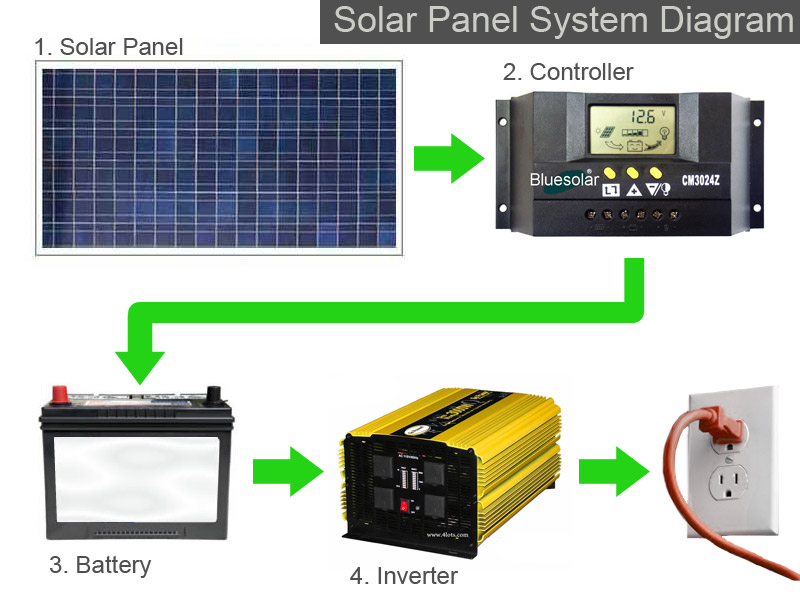
\includegraphics[width=60mm]{system-diagram.jpg} \\
Figure 1: Diagram of the solar 
\end{center}

\section*{Conclusion}

While providing electronics to help improve science and technology education in Africa is noble, doing so requires said electronics to be powered. Thus, it is necessary to provide a consistent and affordable source of energy. Solar panels are clean, sustainable, and relatively cheap sources of energy. A small 2.4 kWh system can provide more than enough energy for the systems needing to be powered. While initial costs can be high, panels have an average life span of 20 plus years. A typical 2.4 kW system costs approximately \$6000 over 20 years (batteries need replacing every 5). However, that cost is spread over that time and is only about \$300 per year. Additionally, extra power generated by the cells can be sold to help further mitigate cost. Overall, the benefits of solar panels outweigh the drawbacks. Thus, solar panels are a worthwhile investment and line up well with goals of this organization.




\end{document}
